\documentclass[a4paper,12pt,twocolumn]{article}

%***************** Packages for Graphics & Figures *******************%
\usepackage{graphicx} %%For loading image files
\graphicspath{ {images/} } %folder-location for images


\newcommand*{\MyPath}{../latex-files}%

\begin{document}

\begin{abstract}
The world we live is a ecosystem which has co-existence of various species in an environment. Interaction between species with its environment are fundamental to survival of species and functioning of the ecosystem. There is an interesting dynamics behind existence of this ecosystem. In ecology, there is system of predator-prey to maintain the ecosystem, where a predator forages on its prey. The predator-prey relationship is substantial in maintaining the equilibrium  between various animal species. Without predators, certain species of prey would force other species to extinction as a result of competition. Without prey, there would be no predators! The key feature of predation thus is the predator's direct impact on the prey population.

Alfred J. Lotka and Vito Volterra proposed set of differential equations to describe the dynamics of biological systems in which two species interact, one as predator and other as prey. Lotka and Volterra equation are \cite{scipy}
 
\end{abstract}

\section{Introduction}

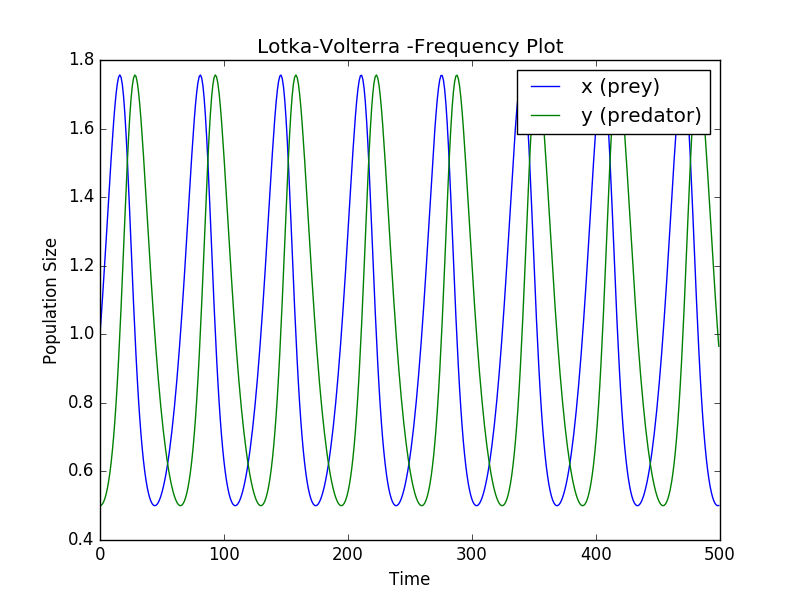
\includegraphics[scale = 0.4]{figure_1}

%  Bibilography
\bibliographystyle{plain}
\bibliography{\MyPath/references/references_LV_model.bib}

\end{document}
